\documentclass[11pt]{article}
%---- defitions ----
\def\Author{Andreas Bock\\
Asbj\o rn Thegler\\
Lasse Dessau
}
\def\Title{\bf Principles of Computer Systems Design\\ {\Large Assignment 1}}
% <Add more defitions here>
%-------------------

%---- packages ----
\usepackage[]{amsmath}
\usepackage[english]{babel}
\usepackage[utf8]{inputenc}
\usepackage{graphicx}
\usepackage{moreverb}
\usepackage{hyperref}
\usepackage{color}
\usepackage{listings}
\usepackage{algorithmicx}
\usepackage{algorithm}
\usepackage{algpseudocode}
\usepackage[T1]{fontenc} % font
\usepackage{program}
\usepackage[top=2in, bottom=0.5in, left=1.4in, right=1.4in]{geometry}
%---- settings ----
% Comments
\newcommand{\comm}[2]{{\sf \(\spadesuit\){\bf #1: }{\rm \sf #2}\(\spadesuit\)}}
\newcommand{\mcomm}[2]{\marginpar{\scriptsize \comm{#1}{#2}}}
\newcommand{\ab}[1]{\mcomm{AB}{#1}} % Andreas Bock

\topmargin=-0.9in % start text higher on page
\textheight=695pt
\setlength{\parindent}{0in}
\definecolor{lightgray}{rgb}{0.9,0.9,0.9}
\renewcommand*\rmdefault{ppl} % font
%-------------------

\begin{document}
\title{\Title}
\author{\Author}
\date{\today}
\maketitle

\section*{Question 1: Serializability \& Locking}

A schedule is conflict serializable if and only if it’s precedence graph is
acyclic. The graphs are computed by drawing arrows from operations in a
transaction $T_j$ that conflicts with an earlier operation in $T_i$.

\subsection*{Schedule 1}

This schedule is not conflict serializable since the precedence graph is
cyclic. In particular:

\begin{itemize}
\item $T_1$ reads $X$ after which $T_2$ wants to write to $X$ resulting in a
read-write conflict.
\item $T_2$ writes $Z$ which $T_3$ then reads resulting in a write-read conflict.
\item $T_3$ reads $Y$ which is then written to by $T_1$ resulting in a
read-write conflict.
\end{itemize}

Schedule 1 cannot possible be generated by strict 2PL since $T_1$ has a shared
lock on $X$ when $T_2$ writes to it.
The precedence graph can be seen in figure \ref{fig:s1}.\\

\begin{figure}[h!]
\begin{center}
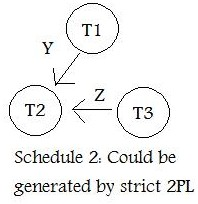
\includegraphics[scale=0.45]{2pl1.jpg}
\caption{Precedence graph for schedule 1.}
\label{fig:s1}
\end{center}
\end{figure}

\subsection*{Schedule 2}

This schedule is conflict serializable since the precedence graph is acyclic.
In particular:

\begin{itemize}
\item $X$ locked by $T_1$ is only accessed in $T_2$ after $T_1$ has committed
and thus released the lock.
\item $Y$ is only accessed by $T_2$.
\item $Z$ exclusively locked by $T_3$ is released prior to $T_2$ acquiring a
shared lock.
\end{itemize}

The locks are acquired and released in the order depicted in figure \ref{fig:acq},
and figure \ref{fig:s2} shows the precedene graph.

\begin{figure}[h!]
\begin{center}
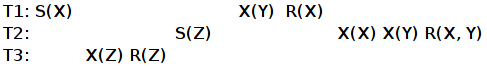
\includegraphics[scale=0.45]{acquisition.png}
\caption{Acquisition on shared/exclusive locks in schedule 2.}
\label{fig:acq}
\end{center}
\end{figure}

\begin{figure}[h!]
\begin{center}
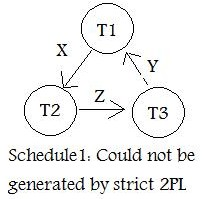
\includegraphics[scale=0.45]{2pl2.jpg}
\caption{Precedence graph for schedule 2.}
\label{fig:s2}
\end{center}
\end{figure}

\section*{Question 2: Optimistic Concurrency Control}

For this question, we refer to the course compendium page 91, where
the \emph{validation conditions} are described. We will refer to the conditions as
1, 2 and 3, respectfully, as listed in the material.

\subsection*{Scenario 1}

$T_1$ finishes before $T_3$ even starts, so we see that\emph{validation
condition 1} holds for this transaction. We check if \emph{validation
condition 2} holds for $T_2$, but since $T_2$ writes to \emph{object 4},
which $T_3$ reads from, it turns out that the condition does not hold.
$T_3$ will have to be \emph{rolled back}.

\subsection*{Scenario 2}

We check if \emph{validation condition 2} holds for $T_1$, but since $T_1$
writes to \emph{object 3}, and $T_3$ reads from it, it turns out that the
condition does not hold. $T_3$ will have to be \emph{rolled back}. We were 
asked for all offending objects, so we will continue checking $T_2$. We
check if \emph{validation condition 3} holds for $T_2$, and since T3 does
not access (read or write) object 8, which is the only object T2 writes to,
the condition holds.

\subsection*{Scenario 3}

We check if \emph{validation condition 2} holds for $T_1$, and since $T_3$
does not read from \emph{object 4}, which is the only object $T_1$ writes to,
the condition holds. We check if \emph{validation condition 2} holds for $T_2$
, and since $T_3$ does not read from \emph{object 6}, which is the only object
$T_2$ writes to, the condition holds. $T_3$ will can be allowed to commit.

\section*{Programming Task}

In this section we go through our implementation and how our choice of
concurrency control protocol adheres to the requirements of
\texttt{acertainbookstore.com}.

\subsection*{Implementation}

As stated in the assignment text, the \texttt{synchronized} keyword has
been removed to allow for finer grained concurrency control by using
appropriate locks.
This has been achieved by using a \href{http://docs.oracle.com/javase/6/docs/api/java/util/concurrent/locks/ReentrantReadWriteLock.html}{\texttt{ReentrantReadWriteLock}}  ,
which allows us to declare read and write locks with the desired semantics.

Our concurrency control protocol is \emph{almost} strict two-phase locking (S2PL).
The only difference is we are more conservative, and have identified the methods
that at \emph{some} point may require a write lock, and made them acquire it
from the start.
In other words, acquisition of the locks follows the diagram from Marcos'
slides (figure ~\ref{fig:lock}).\\

\begin{figure}[h!]
\begin{center}
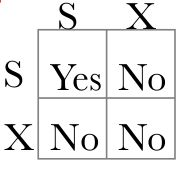
\includegraphics[scale=0.45]{lock.png}
\caption{Locking solution for isolation.}
\label{fig:lock}
\end{center}
\end{figure}

More concretely, this means that methods such as \texttt{getEditorPicks} and
\texttt{getBooks} need only acquire the read lock, while the methods that
need to acquire write locks. Unfortunately, the library
we have used for synchronization does not allow us to upgrade from a read
to a write lock, so one option was to implement our methods in a manner
consistent with the pseudocode described in algorithm
\ref{lst:readwrite}.\\

\begin{algorithm}
\caption{Pseudocode for methods that need to read and write}
\label{lst:readwrite}
\begin{algorithmic}
\Function{readAndWriter}{someParams}\\
\hspace{0.58cm}\Call{acquireReadLock()}{}
\If {requestIsValid}\\
\hspace{1.16cm}\Call{releaseReadLock()}{}
\hspace{1.16cm}\Call{acquireWriteLock()}{}
    \State $result\gets \Call{doWrite}{someParams}$
\Else
    \State $result\gets Error$
\EndIf\\
\hspace{0.58cm}\Call{unlockAcquired()}{}\\
\hspace{0.58cm}\Return $result$
\EndFunction
\end{algorithmic}
\end{algorithm}

It is clear that the method is in no way desirable, as a context switch is 
possible between releasing the read lock and acquiring the write lock and
will render the sanity-check useless.
Instead, our writers are implemented as described in algorithm
\ref{lst:readwrite2}.\\

\begin{algorithm}
\caption{Amended pseudocode for methods that need to read and write}
\label{lst:readwrite2}
\begin{algorithmic}
\Function{readAndWriter}{someParams}\\
\hspace{0.58cm}\Call{acquireWriteLock()}{}
\If {requestIsValid}\\
    \State $result\gets \Call{doWrite}{someParams}$
\Else
    \State $result\gets Error$
\EndIf\\
\hspace{0.58cm}\Call{unlockWriteLock()}{}\\
\hspace{0.58cm}\Return $result$
\EndFunction
\end{algorithmic}
\end{algorithm}

We can, however, expect higher throughput even with this protocol as we now
allow for multiple readers, which is convenient for a book store where you
commonly have several customers browsing the wares.

\subsection*{Testing}

We have added the two required tests described in the assignment text, along
with two other tests for \texttt{getInDemand()} and \texttt{getAverageRating()}
\footnote{Which we have also implemented in the new concurrent bookstore.}.

To use JUnit in a threaded test, we have added two fields,
\texttt{Exception exception} and \texttt{Error error}
to our \texttt{ConcurrentBookStoreTest} class that are initialized
to {\tt null} and server as containers for errors and exceptions thrown by any thread that
JUnit has started. These are therefore declared as \texttt{volatile} to indicate that the 
value may never be cached thread-locally so that threads must write directly to
memory instead.\\
This is due to the fact that JUnit will give a false positive if we simply
use \texttt{assertTrue(...)} in another thread, so we need this mechanism to
catch errors in the threads we spawn.
The \texttt{tearDownAfterClass} will then report the error or exception if one
of these are anything other than \texttt{null}.\\

Finally the assignment text states: "\emph{the clients invoke a fixed number of operations,
configured as a parameter...}". This is not clear to us what is meant by this, as
it seems excessive to create a new class where we translate the parameters (along with
parameters such as \texttt{Set<StockBook>} for \texttt{addBooks}. Instead, we have
designed static nested classes that implement \texttt{Runnable} to cater for the
need for multiple threads.\\

Tests are performed locally.

\subsubsection*{Test 1}

This test has been implemented using two helper classes through the \texttt{Runnable}
interface, and perform the necessary operations on the database. The main thread
then reports if we the stock is consistent.

\subsubsection*{Test 2}

This tests uses the same logic as in test 1, with the exception that we have used
the \texttt{volatile} "trick" described in the introduction.

\subsubsection*{Other tests}

In addition to the two above, we have tested \texttt{getInDemand()} and
\texttt{getAverageRating()}, again by creating static nested classes and
running them as separate threads.\\
To properly test the \texttt{getInDemand()} method we have had to delete
a part of the implementation inherited from \texttt{CertainBookStore} class,
as it simply throws an error if a sale miss occurs. We of course want
to keep the bookstore running even though a customer provokes a sale miss.

\subsection*{Discussion}

%1
As mentioned above, our locking protocol follows conservative S2PL and
is in that sense correct. This can easily be seen by observing that we
acquire all locks in the beginning (for both readers and writers), and
release them just before returning from the method.\\

Furthermore, we cannot deadlock as the necessary 
locks are acquired immediately upon entry of the methods in
\texttt{ConcurrentCertainBookStore}.
This lowers concurrency, as we could have multiple methods (reader or
writers) sharing the read lock for their validation steps.
This is a consequence of the implementation of the synchronization
library we have chosen.

%2
We cannot observe phantoms (i.e. problems pertaining to predicate reads, see page 66
of the course compendium) using conservative S2PL, as we perform all
operations (methods) while holding a read or write lock, and as we are
strict we only release them at the end.

However, had we used proper S2PL, phantoms would still not be a problem since
we want users to see the newest state of the bookstore at all times.
For the sake of argument one solution would to lock the table/database
until the reading transaction has finished. This is not feasible, as we would
then allow users who browse the bookstore to prevent other users to buy.  

%3

Scalability is a problem since we lock \emph{the whole} database when we
want to write. The distinction between readers and writers
allows for multiple reads but not for multiple writers (clients).

If we had implemented locks per table entry we could have
hoped for higher scalability as we could potentially have a writer for each
entry, and would amount to higher levels of concurrency. As it is now
our database locking protocol is preventing us from achieving
the level of concurrency that could theoretically be possible.\\

Further, if we exhibit an influx in the amount of clients buying books,
the write lock will be contended and as a result we could experience
thrashing as described in the course compendium. This makes our
solution less scalable than if we had a lock per entry.\\

%4
Finally, ssuming the cost of implementing such a protocol is reasonable, the
overhead being paid by is minimal compared to the gains in concurrency.
As we mentioned early, this can be seen from the nature of the application
we are building, namely a bookstore. We will expect readers to be manifold
compared to the number of writers (readers = browsing customer, writer = 
buyer), and therefore we except the locking protocol to increase our 
throughput while still providing isolation.

\end{document}
